\subsection{Tracking the Points}
The velocity constraint was furthermore limited to only compute the robot movement from the time left over by the vision algorithm.
It is hence assumed that when the time limit $\Delta t$ is exceeded by the vision algorithm, the result of the process is not used.
The time by which $\Delta t$ is reduced, is calculated on runtime and hence dependent on the time it takes to process the specific image.

The slow data set contains 500 points, the medium, 160, and the fast data set contains 50 points.
In order to minimize the effect of outliers, the number of trials is increased on the data sets which have less data points.

The time to find the marker is measured and the mean processing time is shown in table \ref{tb:mean_processing_time}.
The different backgrounds were tested separately to see if it has any impact.
It can be seen that the Corny detector takes more time on backgrounds such as carpet and mosaik window, as they contain a lot of SIFT features.

\begin{table}[H]
\center
\begin{tabular}{|l|*{3}{D{.}{.}{2}|}}
\hline
Background       & Line  & Circles & Corny  \\ \hline
None             & 30.02 & 39.87   & 234.14 \\ \hline
Many Butterflies & 31.38 & 48.13   & 280.96 \\ \hline
Color Spots      & 32.18 & 42.33   & 262.47 \\ \hline
One Butterfly    & 32.17 & 46.75   & 306.68 \\ \hline
Metal            & 33.31 & 42.02   & 258.56 \\ \hline
Carpet           & 33.09 & 49.52   & 364.25 \\ \hline
Mosaik Window    & 31.35 & 42.64   & 322.83 \\ \hline
Waterbed         & 33.25 & 44.35   & 276.99 \\ \hline
\end{tabular}
\caption{Mean processing time [ms] for the vision algorithms on the different backgrounds.}
\label{tb:mean_processing_time}
\end{table}

The minimum $\Delta t$ was found for the different markers on different backgrounds.
The result of such is seen in table \ref{tb:min_dt_lines}, \ref{tb:min_dt_circles}
%, \ref{tb:min_dt_circles_center}
 and \ref{tb:min_dt_corny}.
The marker speeds were only tested for $\Delta t$ being multiples of 50 milliseconds.

\begin{table}[H]
\center
\begin{tabular}{|c|c|c|c|}
\hline
Background       & Fast & Medium & Slow \\ \hline
None             & 50   & 50     & 50   \\ \hline 
Many Butterflies & 50   & 50     & 50   \\ \hline 
Color Spots      & 50   & 50     & 50   \\ \hline 
One Butterfly    & 50   & 50     & 50   \\ \hline 
Metal            & 50   & 50     & 50   \\ \hline 
Carpet           & 50   & 50     & 50   \\ \hline 
Mosaik Window    & 50   & 50     & 50   \\ \hline 
Waterbed         & 50   & 50     & 50   \\ \hline 
\end{tabular}
\caption{Minimum $\Delta t$ [s] for Lines on different backgrounds with different marker speeds.}
 \label{tb:min_dt_lines}
\end{table}

\begin{table}[H]
\center
\begin{tabular}{|c|c|c|c|}
\hline
Background       & Fast & Medium & Slow \\ \hline
None             & 100  & 50     & 50   \\ \hline 
Many Butterflies & 100  & 50     & 50   \\ \hline 
Color Spots      & 100  & 50     & 50   \\ \hline 
One Butterfly    & 100  & 100    & 100  \\ \hline 
Metal            & 100  & 50     & 50   \\ \hline 
Carpet           & 100  & 100    & 50   \\ \hline 
Mosaik Window    & 100  & 50     & 50   \\ \hline 
Waterbed         & 100  & 50     & 50   \\ \hline 
\end{tabular}
\caption{Minimum $\Delta t$ [s] for Circles tracking four points on different backgrounds with different marker speeds.}
\label{tb:min_dt_circles}
\end{table}

%\begin{table}[H]
%\center
%\begin{tabular}{|c|c|c|c|}
%\hline
%Background & Slow & Medium & Fast \\ \hline
%None & 0.0 & 0.0 & 0.0 \\ \hline
%Many Butterflies & 0.0 & 0.0 & 0.0 \\ \hline
%Color Spots & 0.0 & 0.0 & 0.0 \\ \hline
%One Butterfly & 0.0 & 0.0 & 0.0 \\ \hline
%Metal & 0.0 & 0.0 & 0.0 \\ \hline
%Carpet & 0.0 & 0.0 & 0.0 \\ \hline
%Mosaik Window & 0.0 & 0.0 & 0.0 \\ \hline
%Waterbed & 0.0 & 0.0 & 0.0 \\ \hline
%\end{tabular}
%\caption{Minimum $\Delta t$ [s] for Circles tracking one points on different backgrounds with different marker speeds.}
%\label{tb:min_dt_circles_center}
%\end{table}

\begin{table}[H]
\center
\begin{tabular}{|c|c|c|c|}
\hline
Background       & Slow & Medium & Fast \\ \hline
None             & 250  & 200    & 200\\ \hline 
Many Butterflies & 300  & 300    & 300\\ \hline 
Color Spots      & 300  & 250    & 250\\ \hline 
One Butterfly    & 350  & 350    & 350\\ \hline 
Metal            & 250  & 250    & 250\\ \hline 
Carpet           & 450  & 400    & 400\\ \hline 
Mosaik Window    & 350  & 350    & 300\\ \hline 
Waterbed         & 350  & 300    & 300\\ \hline 
\end{tabular}
\caption{Minimum $\Delta t$ [s] for Corny on different backgrounds with different marker speeds.}
\label{tb:min_dt_corny}
\end{table}

In order to measure the systems ability to track the marker, the distance from the ideal position to the position based on the image marker is measured.
In figure \ref{fig:trackingerror_lines}, \ref{fig:trackingerror_circle} and \ref{fig:trackingerror_corny} is the euclidean max error shown for a range of $\Delta t$ in the range where the algorithm goes from not being able to track the marker to being able to.
%\nikolaj{Conclude something: It can be seen that the Circle detector has a larger deviance from the ideal path than the other detectors.}

\begin{figure}[H]
\centering
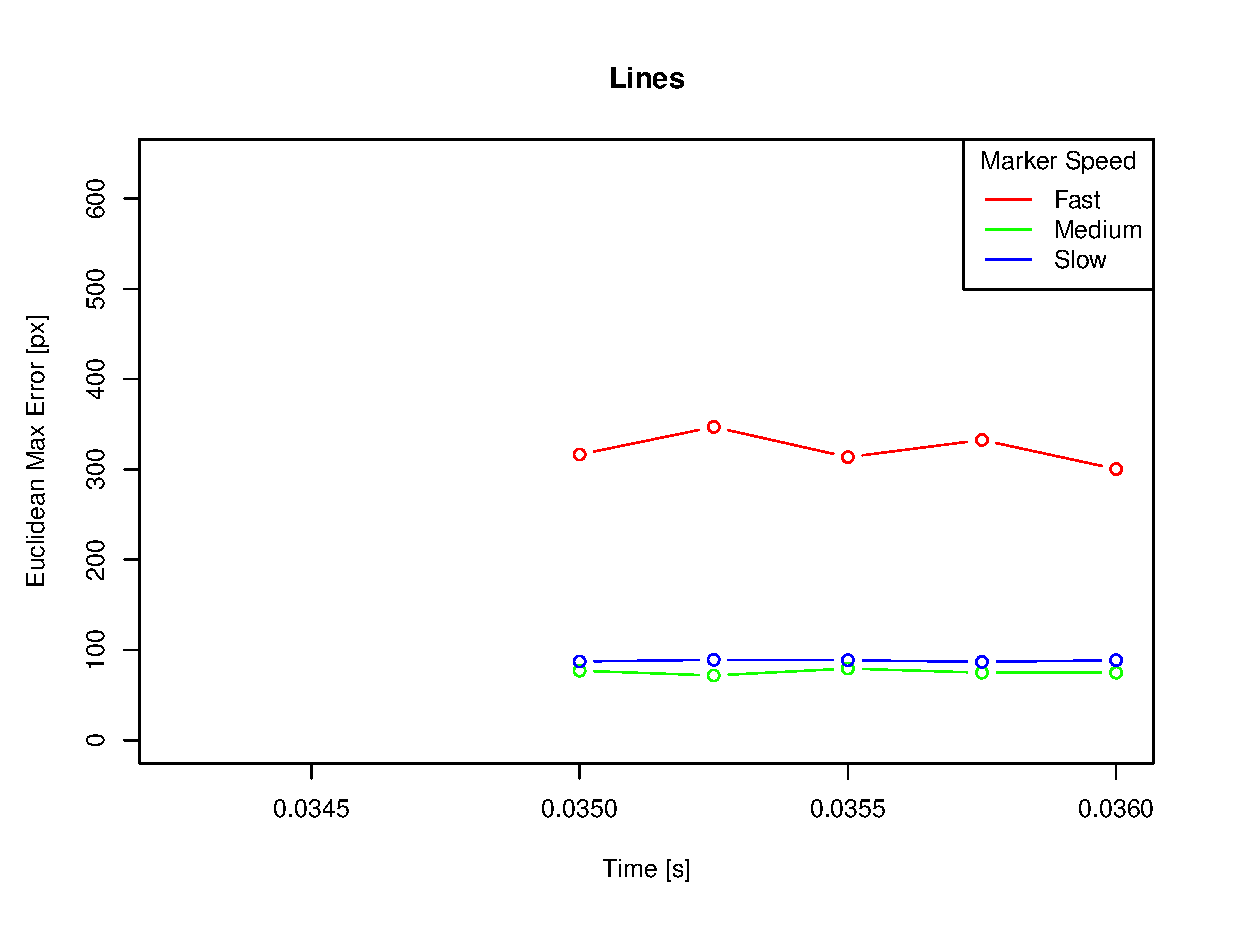
\includegraphics[width= \fullImageWidth]{graphics/robotics/trackingerror_lines}
\caption{Euclidean max error for increasing $\Delta t$ when tracking the line image.}
\label{fig:trackingerror_lines}
\end{figure}

\begin{figure}[H]
\centering
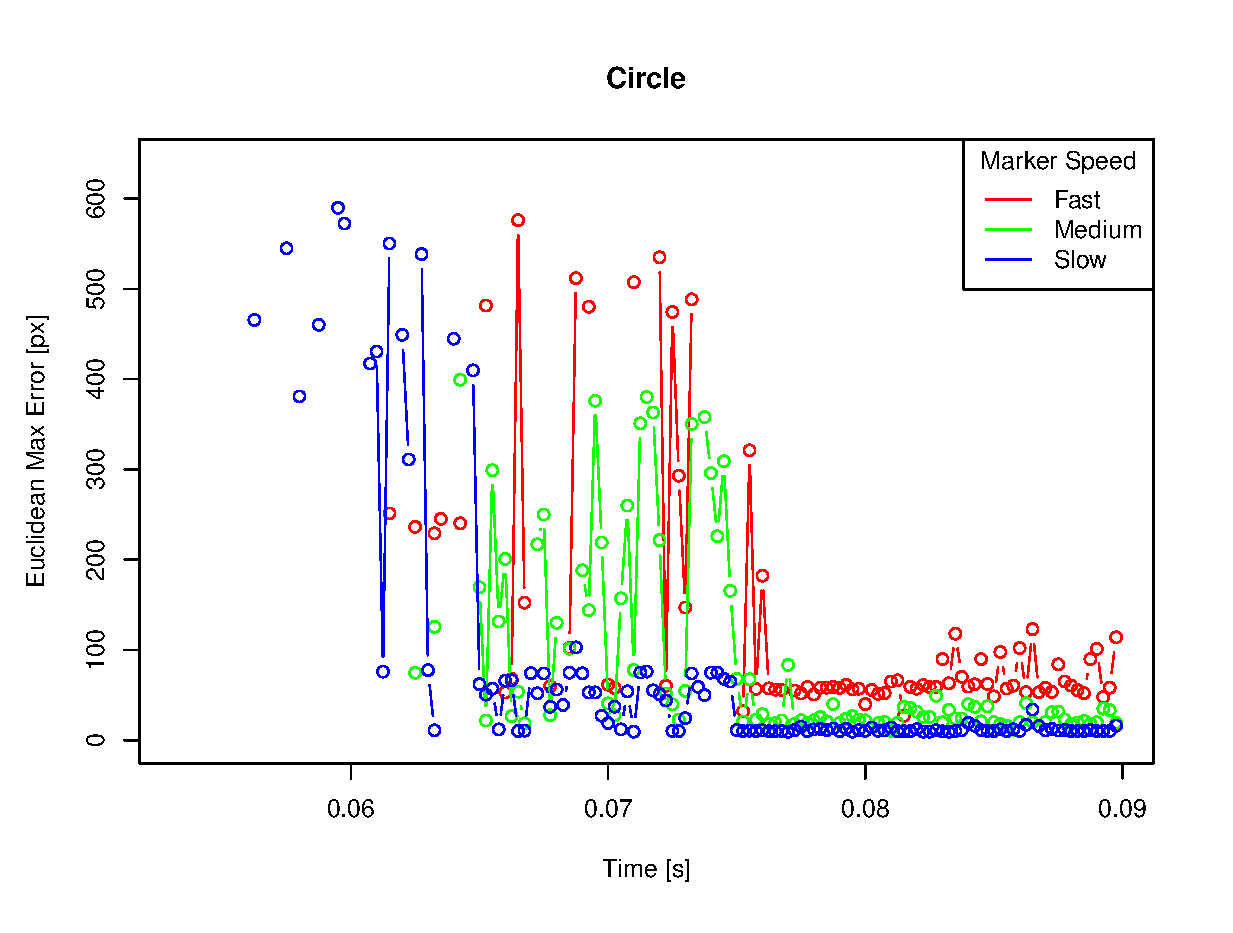
\includegraphics[width= \fullImageWidth]{graphics/robotics/trackingerror_circle}
\caption{Euclidean max error for increasing $\Delta t$ when tracking the circle image.}
\label{fig:trackingerror_circle}
\end{figure}

\begin{figure}[H]
\centering
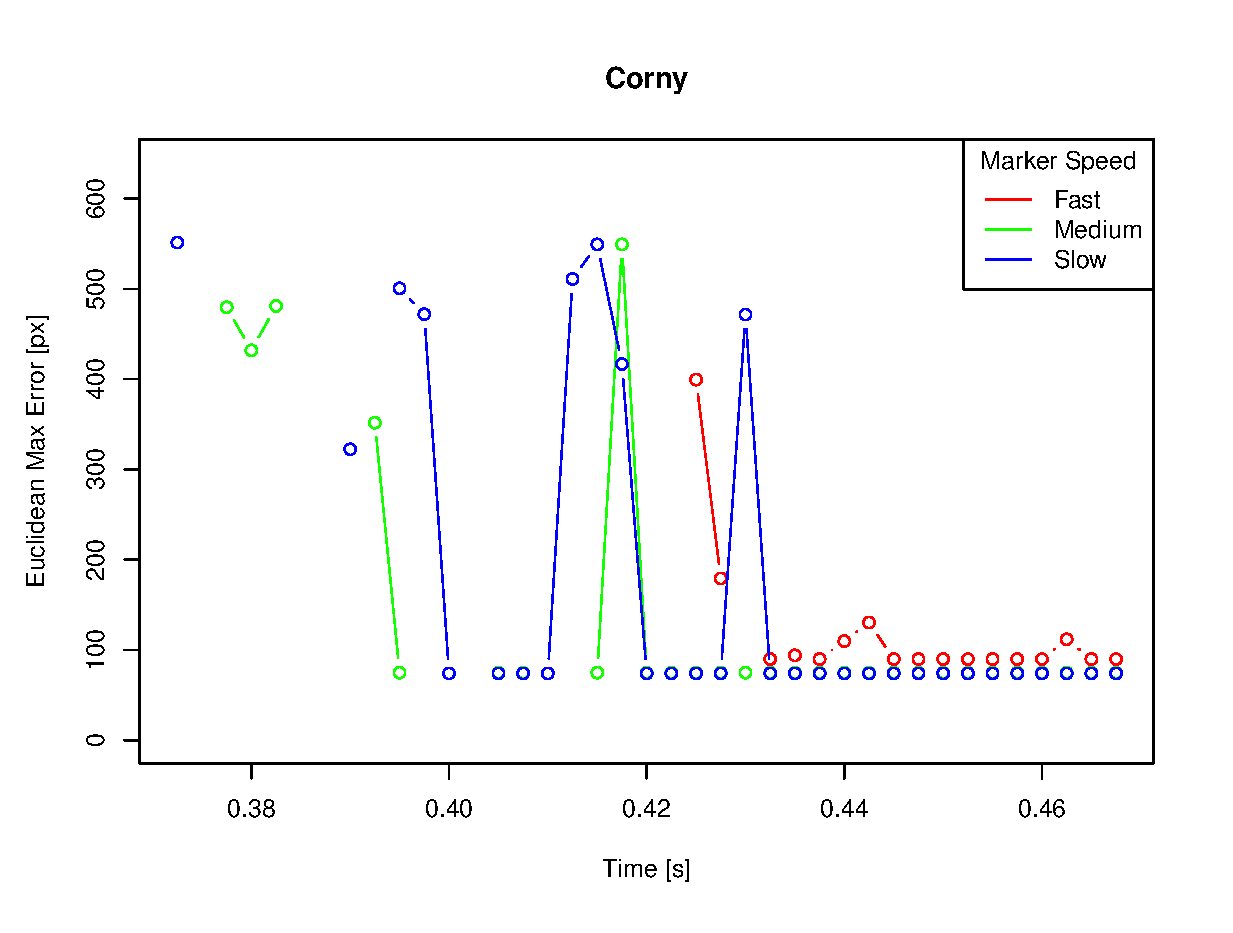
\includegraphics[width= \fullImageWidth]{graphics/robotics/trackingerror_corny}
\caption{Euclidean max error for increasing $\Delta t$ when tracking the corny image.}
\label{fig:trackingerror_corny}
\end{figure}

Note that the data points were sampled with uniform sample steps, but the data points where the program generated 'not track-able' are not plotted.

As can be seen on figure \ref{fig:trackingerror_circle}, the tracking error has a high fluctuation and lack of data points in the range just before the the sufficient time is reached for which the robot can track the marker.
From the figure the minimum time needed to track the marker reliably can be found.
It is furthermore visible that the point from which the marker can be tracked is approximately the same for all three speeds.
Once this point is reached, the error is approximately constant, but dependent on the marker movement speed.
The breakpoint is around $\Delta t = $ 0.078 [s].

The error when tracking the line was found to be more stable.
As seen in figure \ref{fig:trackingerror_lines}, then there is a sharp change from when it is able to track the marker and when not ($\Delta t = $ 0.035 [s]).
The error for the fast marker speed is first stabilised at a low error after $\Delta t =$ 0.045, whereas the other two are constant throughout.
The final error is generally higher than that of the circle marker, but this is also contributed to by the fact that not the precise center of the marker is found in the vision algorithm.

The corny marker using SIFT is the slowest of all the algorithms.
The tracking error of such is seen in figure \ref{fig:trackingerror_corny}.
It can be seen that that the beginning of the graph has a lot of missing data points because the marker left the image while trying to track it.
The algorithm is hence very unstable in the beginning and will only be able to track the marker if it is in some sense 'lucky'.
This problem arises because from the speed optimisation.
Because the algorithm crops the image, then the algorithm will only succeed if the marker does not leave the cropped area.
If it does leave the cropped zone, then the processing of the whole image will take too long for it to be able to finish in time so the robot will stand still.
This also is the reason for why the fast marker movement is not found at all.
The most stable result will hence first be gained when the whole image can be processed in one time-step, $\Delta t$.
The algorithm is however also usable for the slow dataset with $\Delta t > 440ms$ and for the medium likewise.


%The large fluctuation in the maximum error for the Circle algorithm, as seen in figure \ref{fig:trackingerror_circle}, is largely explained by the choice of implementation.
%The default behaviour of the algorithm would only look for circles once in the green channel of the image.
%In worst cases, however, the algorithm finds the hough circles on all three color channels of the image.
%This creates good reasons for the time to variate 

The joint positions and relative joint velocities can be seen in appendix \ref{app:joint_positions_combined_part}.
It can be seen that the circle detector more unstable as joint velocities are several magnitudes higher than on the other markers and the joint positions indicate the robot not settling.